\subsubsection{Descripci\'on} 

\textbf{Direct-optimal basis computation by means of the fusion of Simplification rules, E. Rodr ́ıguez-Lorenzo et.al., Last review Discrete Appl. Math (2017)}

Una vez que hemos conseguido un algoritmo para el c\'alculo del cierre eficiente y optimizado, el siguiente paso para reducir el coste del c\'alculo del cierre es optimizar todo lo posible el sistema implicacional de entrada. Es aqu\'i donde entran en juego nuevos conceptos como son por ejemplo el de base directa \'optima.

K. Bertet \cite{BERTET20102155} propuso la llamada base directa optima como primera aproximaci\'on para reducir el coste del c\'alculo del cierre. Mientras que  K. Adaricheva \cite{Adaricheva} propuso la llamada D-Base como un subconjunto de la base directa optimal. Esto supon\'ia un problema abierto: Mejorar el c\'alculo de estas bases (o algo similar) para reducir el coste del c\'alculo del cierre en consecuencia.

La importancia del c\'alculo de bases directas de sistemas implicacionales ha sido remarcada por diferentes autores en \'areas diferentes ya que su uso es crucial en problemas donde se requiere el c\'alculo de gran cantidad de cierres. Por lo tanto, cuanto mas eficiente sea el c\'alculo de estas bases, mejor rendimiento tendr\'an los m\'etodos de resoluci\'on de esos problemas. 

A continuac\'on se van a detallar algunos de estos conceptos.\\


\textbf{Base}

Un sistema implicacional \( \Sigma \) se dice que es:
\begin{itemize}
    \item una base minimal cuando,  \( para \ todo \ A \to B \in \Sigma \ se \ tiene \ que \ \Sigma \setminus \{A \to B\} \not\equiv \Sigma\)

    \item una base m\'inima cuando,  \( para \ todo \ \Sigma' \equiv \Sigma \ se \ tiene \ que \ |\Sigma| \leq |\Sigma'|\)

    \item una base \'optima cuando,  \( para \ todo \ \Sigma' \equiv \Sigma \ se \ tiene \ que \ \|\Sigma\| \leq \|\Sigma'\| \\ donde \ \|\Sigma\| = 
    \sum_{\substack{A \to B \in \Sigma}} (|A|+|B|) \).
\end{itemize}

\textbf{Directo}

Un sistema implicacional \( \Sigma \) se dice que es directo cuando, \( para \ todo \ X \subseteq S \ se \ tiene \ que \\ X^+_{\Sigma} =  X \cup \bigcup\{ B | A \to B \in \Sigma \ para \ algun \ A \subseteq X \} \). Esto se traduce en que se puede calcular el cierre de un conjunto de atributos con una sola pasada y que ninguna de las implicaciones puede ser eliminada sin perder esta propiedad.

Por tanto, ya se esta en condiciones de conocer que es una base directa \'optima.\\

El teorema 2 de \cite{DO2} nos dice que: 
Para cualquier sistema impicacional \(\Sigma\), existe un \'unica base directa \'optima \(\Sigma_{DO}\) tal que \(\Sigma \equiv \Sigma_{DO} \)\\

Como soluci\'on al c\'alculo de bases directas optimas se ha implementado el algoritmo desarrollado por  E. Rodr\'iguez-Lorenzo et al. \cite{DO2}, llamado [SLgetdo] en el cu\'al se aplican las reglas de L\'ogica de Simplificaciones \(\textbf{SL}_{FD}\). Una primera aproximaci\'on  fue el algoritmo desarrolado tambi\'en por E. Rodr\'iguez-Lorenzo et al. \cite{doSimp}, llamado [doSimp] tambi\'en basado en la L\'ogica de Simplificaciones, apicando la simplificaci\'on (Si-Eq) y la composici\'on (Co-Eq) para simplifcar el sistema implicacional, [sSimp] para completarlo y (rSi-Eq) y (Co-Eq) para optimizar el resultado final. Este primer algoritmo no se ha implementado en el proyecto ya que [SLgetdo] lo mejora, reduciendo el n\'umero de pasos a dos, as\'i como el tama\~no de las bases directas generadas hasta alcanzar la \'optima.
\newpage
\subsubsection{C\'odigo} 
\lstinputlisting{r_code/DO_IS.R}
\newpage
\subsubsection{Ejemplo} 
A continuaci\'on, se muestra un ejemplo del c\'alculo de una base directa optima a partir del siguiente conjunto de implicaciones: 
\begin{figure}[H]
    \centering
    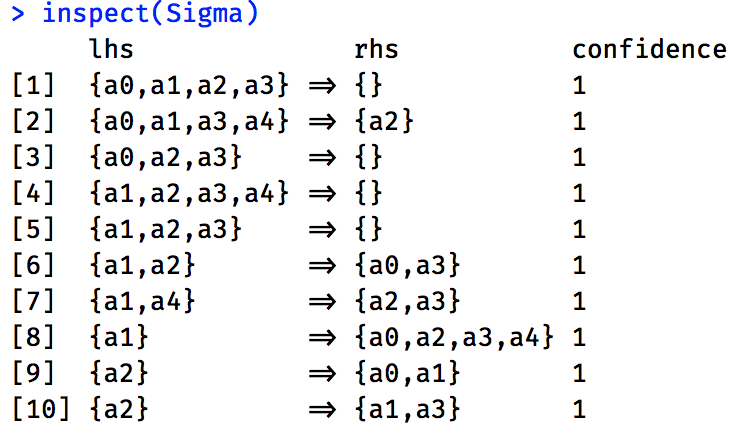
\includegraphics[scale=0.75]{do_1}
    \caption{Ejemplo SLgetdo 1}
    \label{fig:do_1}
\end{figure} 

Aqu\'i se puede ver el resultado:
\begin{figure}[H]
    \centering
    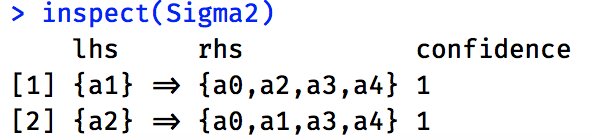
\includegraphics[scale=0.75]{do_2}
    \caption{Ejemplo SLgetdo 2}
    \label{fig:do_2}
\end{figure} 
Y, como era de esperar, el hecho de usar una base directa optima para el c\'alculo del cierre reduce consideradamente los tiempos de ejecuci\'on incluso en ejemplos tan peque\~nos como este, d\'onde el c\'alculo es practicamente inmediato.
\begin{figure}[H]
    \centering
    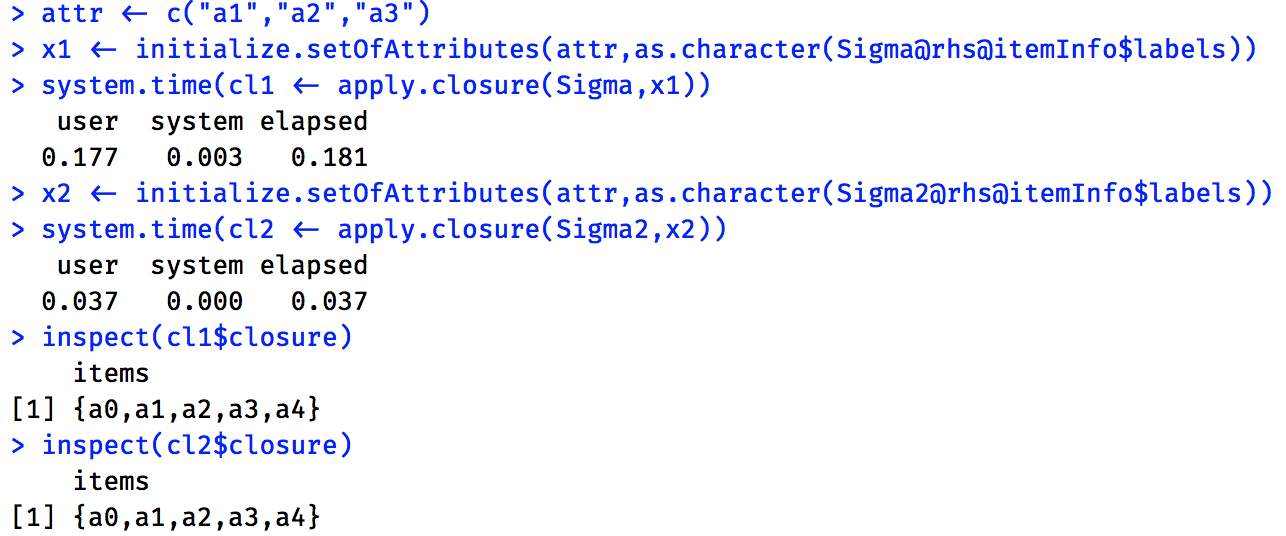
\includegraphics[scale=0.75]{do_3}
    \caption{Comparativa del c\'alculo del cierre a partir de una base DO}
    \label{fig:do_3}
\end{figure} 

Esta reducci\'on de tiempo se acent\'ua conforme crece el tama\~no del conjunto de implicaciones.

Si se tiene en cuenta que para resolver determinados problemas, el c\'alculo de multitud de cierres (del orden de millones) es parte fundamental,\cite{Adaricheva} el impacto de cualquier peque\~na mejora en el c\'alculo de cada uno de esos cierres, puede suponer una diferencia abismal. De ah\'i radica la importancia de este algoritmo.

% \subsubsection{Comparativa/Versiones} 